\documentclass{beamer}

\usepackage[utf8]{inputenc}
\usepackage[ngerman]{babel}

\title{Sweepline Algorithmen - Linienschnitte}
\author{Paul Jungeblut}
\date{2. Juli 2014}

\begin{document}

\selectlanguage{ngerman}

\begin{frame}
\titlepage
\end{frame}

\section{Sweepline}
\begin{frame}{Sweepline - Was ist das?}
	\begin{block}{Sweepline} 
		\begin{itemize}
			\item Häufige Methode zum Lösen geometrischer Probleme
			\item Gesamte Ebene wird mit einer Linie gescannt (Scanline)
			\item Nur an bestimmten, wichtigen Punkten (Events) muss etwas getan werden
		\end{itemize}
	\end{block}
	\begin{exampleblock}{Beispiele}
		\begin{itemize}
			\item Graham-Scan, Sweepline scannt um einen Punkt rotierend
			\item Closest-Pair, klassisch
		\end{itemize}
	\end{exampleblock}
\end{frame}

\subsection{Problem}
\begin{frame}{Problemstellung}
	\begin{block}{Aufgabe}
		\begin{itemize}
			\item $n$ Strecken in der Ebene, jeweils gegeben durch die beiden Endpunkte
			\item \textbf{Aufgabe:} Finde alle Schnittpunkte
		\end{itemize}
	\end{block}
	
	\begin{block}{Vereinfachungen}
		\begin{itemize}
			\item keine zwei End-/Schnittpunkte haben die gleiche x-Koordinate
			\item kein Endpunkt liegt auf einer anderen Strecke
			\item max. 2 Strecken schneiden sich in einem Punkt
		\end{itemize}
	\end{block}
\end{frame}

\begin{frame}{Naiver Ansatz}
	\begin{exampleblock}{Erinnerung}
		$Schnitt(p_1, p_2, p_3, p_4) = \newline
		\hspace*{1cm} ccw(p_1, p_2, p_3) \cdot ccw(p_1, p_2, p_4) \le 0 \wedge \newline
		\hspace*{1cm} ccw(p_3, p_4, p_1) \cdot ccw(p_3, p_4, p_2) \le 0$
	\end{exampleblock}
	\begin{figure}
		\vspace{-2.5cm}\hspace*{6cm}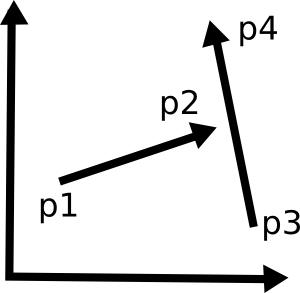
\includegraphics[width=2cm]{intersect2.png}\\
	\end{figure}
	\hspace{3cm}
	\begin{block}{Algorithmus}
		\begin{itemize}
			\item Teste für je zwei Strecken, ob sie sich schneiden
			\item Berechne Schnittpunkt (LGS)
			\item Laufzeit: $O\left(n^2\right)$
		\end{itemize}
	\end{block}
\end{frame}

\begin{frame}{Bentley–Ottmann Algorithmus}
	\begin{block}{Idee}
		\begin{itemize}
			\item Lasse Sweepline $L$ von links nach rechts über die Ebene laufen.
			\item Zu jedem Zeitpunkt schneidet S eine Teilmenge der Strecken. Die vertikale Anordnung verändert sich dabei nur bei einem Schnittpunkt.
			\item Events sind
				\begin{itemize}
					\item noch nicht gescannte Endpunkte
					\item Schnittpunkte von Strecken, die in der vertikalen Anordnung nebeneinander liegen
				\end{itemize}
		\end{itemize}
	\end{block}
\end{frame}

\begin{frame}{Bentley–Ottmann Algorithmus}
	\begin{block}{Algorithmus - Initialisierung}
		\begin{enumerate}
			\item Erstelle Priority Queue $pq$ für zukünftige Events, priorisiert nach x-Koordinate. $pq$ enthält zu Beginn alle Endpunkte.
			\item Erstelle Set $T$ für vertikale Anordnung der Schnittpunkte zwischen den Strecken und der Sweepline. Sortierung nach y-Koordinate. Zu Beginn leer.
			\item Solange $pq$ nicht leer ist, entferne erstes Element aus $pq$. 3 Fälle treten auf:
		\end{enumerate}
	\end{block}
\end{frame}

\begin{frame}{Bentley–Ottmann Algorithmus}
	\begin{block}{Linker Endpunkt einer Strecke $s$:}
		\begin{itemize}
			\item Füge $s$ in $T$ ein.
			\item Suche Strecken $r$ und $t$ direkt über und unter $s$. Falls ihr Schnittpunkt als Event in $pq$ liegt, entferne ihn.
			\item Falls $s$ die Strecken $r$ oder $s$ schneidet, füge die Schnittpunkte in $pq$ ein.
		\end{itemize}
	\end{block}
	\begin{figure}
		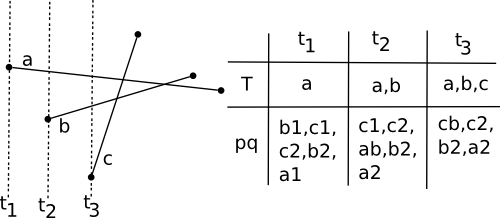
\includegraphics[scale=0.8]{insert.png}\\
	\end{figure}
\end{frame}

\begin{frame}{Bentley–Ottmann Algorithmus}
	\begin{block}{Rechter Endpunkt einer Strecke $s$:}
		\begin{itemize}
			\item Suche Strecken $r$ und $t$ direkt über und unter $s$. Falls sie sich noch schneiden, füge Schnittpunkt zu $pq$ hinzu.
			\item Entferne $s$ aus $T$.
		\end{itemize}
	\end{block}
	\begin{figure}
		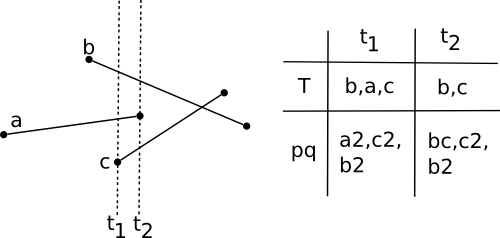
\includegraphics[scale=0.8]{remove.png}\\
	\end{figure}
\end{frame}

\begin{frame}{Bentley–Ottmann Algorithmus}
	\begin{block}{Schnittpunk zweier Strecken $s$, $t$:}
		\begin{itemize}
			\item Tausche Positionen von $s$ und $t$ in $T$.
			\item Finde Strecken $o$ und $u$ darüber und darunter. Entferne Schnittpunkte mit diesen, füge neue ein.
		\end{itemize}
	\end{block}
	\begin{figure}
		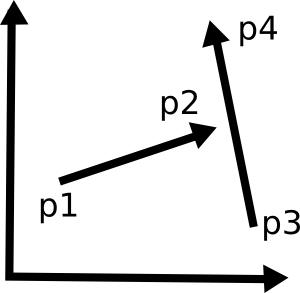
\includegraphics[scale=0.8]{intersect.png}\\
	\end{figure}
\end{frame}

\end{document}